\documentclass[12pt, letterpaper]{article}
\usepackage[utf8]{inputenc}
\usepackage{longtable}
\usepackage{graphicx}
\usepackage{verbatim}
\usepackage{multirow}

\graphicspath{ {images/} }

\title{Recognition of emotions in speech:\\overview and implementation}
\author{Aydar Musin\\Supervisor: prof. Maxim Talanov}
\date{June 2015, Innopolis University}

\begin{document}

\begin{titlepage}
\maketitle
\end{titlepage}

\begin{abstract}
In this paper will be considered studies on recognition of emotions in speech, distinguished their techniques, advantages and disadvantages. Then will be offered own simple implementation of the recognition system.
\end{abstract}

\section{Introduction}
Obviously, people express emotions not only by facial expressions and gestures. Emotions are also pronounced in speech. When somebody is excited his voice pitch is increasing, temp of speech increases and decreases length of syllables. Such characteristics and many others described in many studies. 

People can recognize emotion despite other language, age and gender of speaker. It means that there are some dynamics of characteristics for each emotion. And it is possible to implement the system capable for emotion recognition regardless of speech language, speaker's age and gender.

Why recognition of emotions from speech is useful? Speech emotion recognition has many application areas. The most evident of them: robots and improving the quality of customer service.

For robots which are working in the social environment, is important to have such mechanisms. It refers to affective computing approach. Affective computing is the study and development of systems and devices that can recognize, interpret, process, and simulate human affects\cite{affective}. This approach emphasizes importance of emotions for robot. And justifies it by example of importance emotions for human. Because emotions for people help to interact with others, emotional coloring of facts gives better memorization, it helps to decision making, internal processes regulation depends on emotional state.

Firstly, emotion recognition system for robot can help to improve decision making system. Because there are situations when a robot needs to take into account human emotions. In addition, identifying the features of emotions allows us to understand how to generate emotional speech. If robot has option of emotional speech generating, it will help him to interact with people better, beacuse robots with emotional speech are more people-friendly. In total, people's emotions understanding and emotional speech generation for robot helps to be people-friendly and more effective. Already exist robots which have such options. For example, Pepper:
\begin{quote}
	Pepper is the first humanoid robot designed to live with humans. At the risk of disappointing you, he doesn't clean, doesn't cook and doesn't have super powers... Pepper is a social robot able to converse with you, recognize and react to your emotions, move and live autonomously\cite{pepper}
\end{quote}
Closer to reality application of this system is within an estimation of customer service quality. For example, call-centers have records of conversations. And for operator's work estimation we can identify expressive conversations and analyze them. It can be used with conjunction of speech recognition. For analyzing customer calls, speech can be analyzed by sound characteristics and speech phrases.
%%%%%%%%%%%%%%%%%% Examples!!!!!!!!!!!!!!!

\section{The main goal and problem}

There are many studies which deal with recognition of emotions in speech. Main differences between them in using different:
\begin{itemize}
	\item Acoustics characteristics
	\item Features
	\item Classification techniques
	\item Recognizable emotions
\end{itemize}

Exist papers where are considered these differences, but often there are discussed only sound characteristics, features, and classification problems. Few works which compare influence of selected emotions to the system accuracy. The main goal of this work is to consider differences of several studies on this topic and to offer own simple implementation. Then with testing check how to influence selected emotions to accuracy.
In addition there are some other problems such as: sound characteristics extraction, noise removing, dividing speech to phrases. Will be given examples of libraries and algorithms for solving these problems.

\section{Overview}
\subsection{Acoustic characteristics}
Before we consider a few studies, let's consider some acoustic characteristics:
\begin{itemize}
	\item Pitch or fundamental frequency
	\item Loudness or intensity
	\item Formants
	\item MFCC (Mel-frequency cepstrum coefficients)
\end{itemize}

\subsubsection{Pitch}
Human speech frequency is approximately in the range of 300 to 3400 Hz. The fundamental frequency of speech for male from 85 to 185 Hz, for female from 165 to 255.
\begin{quote}
The fundamental frequency, often referred to simply as the fundamental, is defined as the lowest frequency of a periodic waveform. In terms of a superposition of sinusoids (e.g. Fourier series), the fundamental frequency is the lowest frequency sinusoidal in the sum \cite{wiki1}.
\end{quote}

\subsection{Loudness}
It is sound characteristic which as well carries useful information for recognition, but it should be used very carefully. Because values of this characteristic depends on record quality and speaker's manner of speaking.
\begin{quote}
Loudness is the characteristic of a sound that is primarily a psychological correlate of physical strength (amplitude). More formally, it is defined as "that attribute of auditory sensation in terms of which sounds can be ordered on a scale extending from quiet to loud".
Loudness, a subjective measure, is often confused with objective measures of sound strength such as sound pressure, sound pressure level (in decibels), sound intensity or sound power.\cite{wiki_loudness}
\end{quote}

\subsubsection{Formant and MFCC}
The most frequently in studies used only pitch and loudness. Although formant and MFCC characteristics also useful.
\begin{quote}
Formant is a range of frequencies of a complex sound in which there is an absolute or relative maximum in the sound spectrum". In speech science and phonetics, however, a formant is also sometimes used to mean an acoustic resonance of the human vocal tract.\cite{wiki2}
\\
\\
In sound processing, the mel-frequency cepstrum (MFC) is a representation of the short-term power spectrum of a sound, based on a linear cosine transform of a log power spectrum on a nonlinear mel scale of frequency\cite{wiki3}.
\end{quote}


\subsection{Features}
For emotion classification using acoustic characteristics is necessary to extract some features of these characteristics for every emotion. We extract and compute emotion features from training set to use it for classification. And classification is done:
\begin{enumerate}
	\item Extract features from processed speech
	\item Compare extracted features with emotion's features
\end{enumerate}

Features can be divided to two types by how to compute and how to compare them:
\begin{itemize}
	\item speaker-dependent
	\item speaker-independent
\end{itemize}

\subsubsection{Speaker-dependent features}
Firstly, with speaker-dependent features we need a divided training set for every person. And compute features for every person. During classification we need to compare extracted features with personal features. Advantages of this technique: would be increment of precision. Because unlike speaker-independent features here is less variation of characteristics. These features based on some average values. For example: average pitch, average intensity, pitch range, intensity range. And they are different for every person. That is why it is not a universal technique because requires statistics keeping for each person. And it is can be applied only in a few cases.
\subsubsection{Speaker-independent features}
Unlike a previous technique here divided training set is not required. But the accuracy of classifying depends on number of speech records and number of speakers represented in the training set. Features based on speech signal dynamics, also some average values. For example, pitch DDS (explanation further), intensity DDS, average phrase duration, etc.


\subsection{Classification}
From one side classification problem in this case very similar to other problems. And it can be solved by Binary decision tree, Naive Bayes classifier, ANN. But from other side it has some specific points caused by emotions similarity and ambiguity. Classification techniques described in detail in the paper: \cite["Speaker Emotion Recognition Based on Speech Features and Classification Techniques"]{SirishaSirvinasSiva}. So let's consider some of them.
\subsubsection{Binary   Decision Tree}
In computer science, a binary decision tree is a data structure that is used to represent a Boolean function. A Boolean function can be represented as a rooted, directed, acyclic graph, which consists of several decision nodes and terminal nodes.
\\
\\
\emph{Advantages:} easy implementation, easy explanation of input and output relationship Can handle high dimensional data Easy to interpret for small sized trees The learning and classification steps of induction are simple and fast Accuracy is comparable to other classification techniques for many simple data sets Convertible to simple and easy to understand classification rules.
\\
\\
\emph{Disadvantages:} decision-tree learners can create overcomplex trees that do not generalize the facts and figures well. Decision trees can be unstable because small variations in the facts and figures might outcome in a absolutely different tree being developed. This difficulty is mitigated by using decision trees inside an ensemble. The difficulty of discovering an optimal decision tree is known to be NPcomplete under several facets of optimality and even for easy concepts. Consequently, functional decision-tree learning algorithms are founded on heuristic algorithms such as the greedy algorithm where locally optimal decisions are made at each node. Such algorithms will not assurance to return the globally optimal decision tree. There are concepts that are hard to discover because decision trees do not articulate them effortlessly, such as XOR, parity or multiplexer troubles. conclusion tree learners conceive biased trees if some categories dominate. It is thus suggested to balance the dataset prior to fitting with the conclusion tree
\\
\\
\subsubsection{Artificial Neural Network}
In machine learning and cognitive science, artificial neural networks (ANNs) are a family of statistical learning models inspired by biological neural networks (the central nervous systems of animals, in particular the brain) and are used to estimate or approximate functions that can depend on a large number of inputs and are generally unknown. Artificial neural networks are generally presented as systems of interconnected "neurons" which send messages to each other. The connections have numeric weights that can be tuned based on experience, making neural nets adaptive to inputs and capable of learning.
\\
\\
\emph{Advantages:} Neural systems are rather easy to implement (you do not need a good linear algebra solver as for examples for SVNs). Neural networks often exhibit patterns alike to those exhibited by humans. although this is more of interest in cognitive sciences than for functional examples.
\\
\\
\emph{Disadvantages:} Long preparing time, Neural systems can't be retrained. Provided that you include information later, this is just about difficult to add to an existing system. Taking care of time arrangement information in neural systems is an exceptionally confounded point.
\\
\subsubsection{Naïve Bayes classifier}
The Naive Bayes Classifier procedure is reliant upon the purported Bayesian hypothesis and is particularly suited when the dimensionality of the inputs is high. Notwithstanding its effortlessness, Naive Bayes can frequently outflank more refined grouping strategies.
\\
\\
\emph{Advantages:} fast to train (single scan). Fast to classify Not sensitive to irrelevant features Handles real and discrete data Handles streaming data well.
\\
\\
\emph{Disadvantages:} assumes independence of features



\subsection{Selected emotions for recognizing}
Accuracy of recognition depends not only on extracted features and used classifier, also it depends on recognized emotions. It is caused by that some emotions are very similar. And to improve classifying similar emotions is necessary improve features extraction and classifier. More emotions- less accuracy. That is why it is a trade-off between recognizable emotions and accuracy.
\begin{figure}[t]
	\centering
	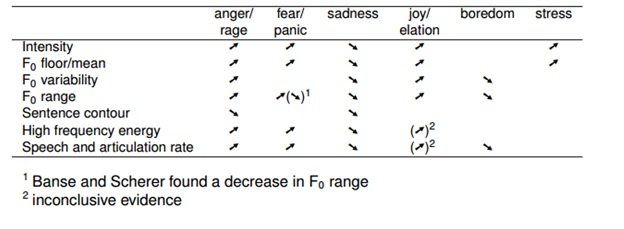
\includegraphics[scale=0.8]{emotion-table-example}
	\caption{Sound characterisstics for emotions [1]}
	\label{fig:emotion-table-example}
\end{figure}

For example, at the Figure 1 showed some features of emotions. And we can see that some emotions very similar(anger-joy,sadness-boredom). Although number of emotions is not so large. But with increasing number of emotions, also increases intersections between emotions on features. So it's important to define emotions which is needed for particular task
\subsection{The general trends of recent studies}
The most of works more and more are using speaker-independent features. By identifying features based on dynamics of characteristics. It caused by that it is universal approach and it has more application domains.

Classification problem is solving by various techniques such as: SVM(Support vector machine), kNN, Hidden Markov Models, ANN. Although more simple solution such as Binary decision tree works not so worse.

\begin{table}[h]
	\begin{tabular}{|p{3cm}|p{3cm}|p{3cm}|p{3cm}|p{3cm}|}
		Title & Authors & Sound characteristics and features & Classification methods & Emotions \\ \hline
		Real-time automatic emotion recognition
		from speech & Britta Wrede, Elisabeth André & pitch, loudness, spectrum, MFCC, speaking rate. DDS, mean, median, varince values for characteristics & SVM, Naive Bayes & positive-active, negative-active, positive-passive, negative-passive\\ \hline
		The production and recognition of emotions in
		speech: features and algorithms & Pierre-Yves Oudeyer & pitch, loudness. Mean, variance, contour rising or falling features. & k-NN, SVM, Naive Bayes& Calm, anger, sadness, comfort, happiness\\ \hline
		Speech Emotion Recognition Using Hidden Markov Models & Albino Nogueiras, Asunción Moreno, Antonio Bonafonte, and José B. Mariño & pitch, energy & Hidden Markov Models & Surprise, Joy, Anger, Fear, Disgust, Sadness, Neutral \\\hline
	\end{tabular}
	\caption{Comparison of some studies}
	\
\end{table}
\section{Implementation}
\subsection{The goal in general}
The main goal is to implement simple recognition system. The program should have option of emotion recognizing from sound file or microphone. Also, it should be resistant to interference and noise. Implementation will be carried out using C\# programming language.

Implementation can be divided to four steps:
\begin{enumerate}
	\item Extracting sound characteristics from sound file or microphone
	\item Speech splitting to phrases or words
	\item Feature extraction and analyzing
	\item Classification
\end{enumerate}

\begin{figure}
	\centering
		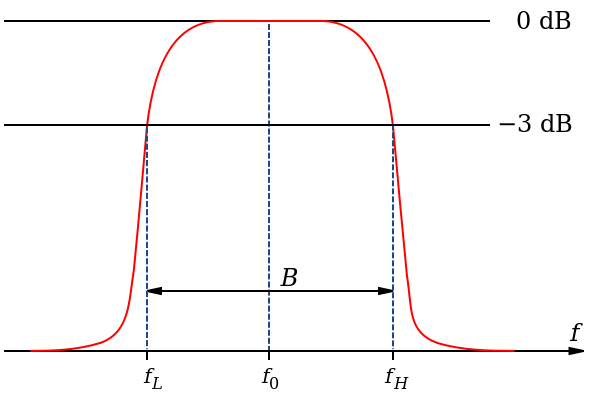
\includegraphics[scale=0.7]{images/pass-band-filter.png}
	\caption{Pass-band filter}
	\label{fig:pass-band-filter}
\end{figure}

\subsubsection{Extracting sound characteristics}

Firstly, is important to note, that is needed only sound characteristics of voice. And to avoid wrong results, sound should be filtered before analyzing. Filtering is important not only for extraction correct voice characteristics, also because it allows to divide voiced and unvoiced intervals of speech.
\\

To retrieve sound characteristics using C\# one can use these libraries:
\begin{itemize}
	\item NAudio (http://naudio.codeplex.com)
	\item Bass Audio library (http://naudio.codeplex.com)
\end{itemize}

But these libraries provide only sound signal receiving from file or microphone. And to get sound characteristic, for example pitch, we have to implement also Fast Fourier Transform function. Also, we have to implement filtering function. For example, simplest filtering can be implemented as pass-band filter. 

Pass-band filter just establish range of signal values, and if signal values go beyond they will be ignored.(Figure 2)
\\
There is also software package which fits our goals - PRAAT. It is often used for speech analyzing and contains all needed functions:
\begin{itemize}
	\item Get fundamental frequency (pitch)
	\item Get loudness
	\item Get spectrogram
	\item Get formant
	\item Filtering function
\end{itemize}

That are functions that we will use, but package contains a lot more functions. And for using all function it has own script language. 

For filtering in the package is using \textit{Remove noise} function. Which consists of pass-band filter and special functions for white noise removing.

Eventually, using PRAAT we will get from sound file these characteristics:
\begin{itemize}
	\item Pitch, or F0
	\item Loudness, or intensity
	\item Formant (F1, F2, F3)
	\item Center of gravity of spectrogram
\end{itemize}
Graphics for these characteristics represented in the Figure 3. We can see that there are intervals where values are equal to zero. It is the result of filter working. When pitch (F0) goes beyond human speech frequency range, all values are assigned to zero.
\begin{figure}
	\centering
		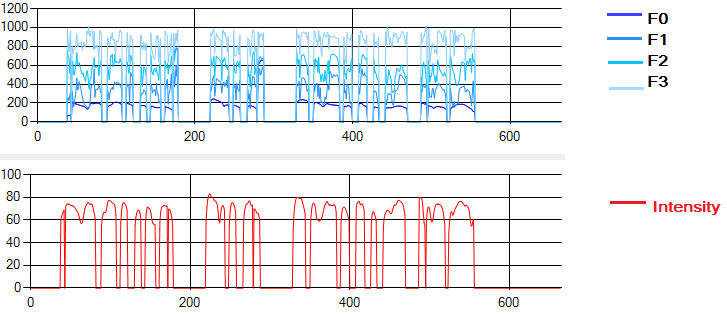
\includegraphics[scale=0.8]{images/sound-characteristics.png}
	\caption{Extracted sound characteristics}
	\label{fig:sound-characteristics}
\end{figure}

\subsubsection{Dividing speech to phrases}

When people are speaking, they express emotions by changing sound characteristics of phrases or words. And for accurate recognition is needed to divide speech to phrases and analyze them separately.

It is worth noting, that precise dividing is impossible without filtering. That is why successfulness of  this step related with previous step. In output from previous step we get set of characteristics where silence intervals marked as zeros. So, algorithm can be as follows: 

 \begin{itemize}
	 \item Until zero value, collect phrase values
		\item After zero value, ends with this phrase and go to the next
 \end{itemize}

But problem with this in appearing of zeros in the middle of
the phrase. And to solve this problem we should set the minimum length of zeros between phrases. At the Figure 4 is shown speech divided to phrases, and within phrase exist intervals of zeros but they are slight. 

So after two steps in the output is received set of sound characteristics and phrase pointers. It is now necessary to extract features for classification.
\begin{figure}
	\centering
		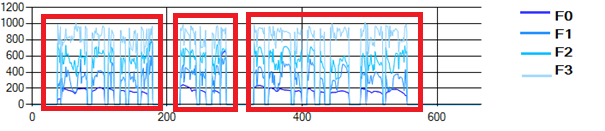
\includegraphics[scale=1]{images/phrases.png}
	\caption{Speech divided to phrases}
	\label{fig:phrases}
\end{figure}
\\
\\
\\
\\
\\
\\

\subsection{Features extraction}

\begin{table}

\begin{tabular}{|p{2.2in}|p{2.2in}|} 
\hline
\multirow{3}{*}{Pitch (F0) }& Variance \\ \cline{2-2}
													& Range \\ \cline{2-2} 
													& DDS \\ \hline 
Formant 1 (F1) & DDS \\ \hline 
Formant 2 (F2) & DDS \\ \hline 
Formant 2 (F3) & DDS \\ \hline 
\multirow{3}{*}{Loudness (Intensity) } & Variance \\ \cline{2-2}
																		& Range \\ \cline{2-2}
																		& DDS \\ \hline 
\multirow{2}{*}{Time} & mean phrase duration \\ \cline{2-2} 
 & mean silence duration \\ \hline 
Spectrogramm & Center of gravity (centroid) \\ \hline 
\end{tabular}
	\caption{Using features}
	\label{Using features}
\end{table}
\emph{Variance.} It can be calculated by standard deviation of set:
\begin{center}
\[V=\sqrt{
\sum_{i=0}^{n}{
               (x_i-\overline{x})^2
               }
}
\]
 where  $\overline{x}$ is average of set\\
\end{center}
\emph{Range.} It is difference between maximum and minimum
\\\\
\emph{DDS (Difference-Distance-Slope)} The idea of this feature taken from\\ \cite["Real-time automatic emotion recognition
from speech"]{brittaelizabet}\\ It is calculating for each phrase (Example in the Figure 5). Then for a whole speech calculate average values of DDS.
\begin{itemize}
	\item Find local $maximum$ and $minimum$ elements for phrase
	\item $difference=maximum-minimum$
	\item $distance=maximum_{position}-minimum_{position}$
\end{itemize}

\begin{figure}
	\centering
		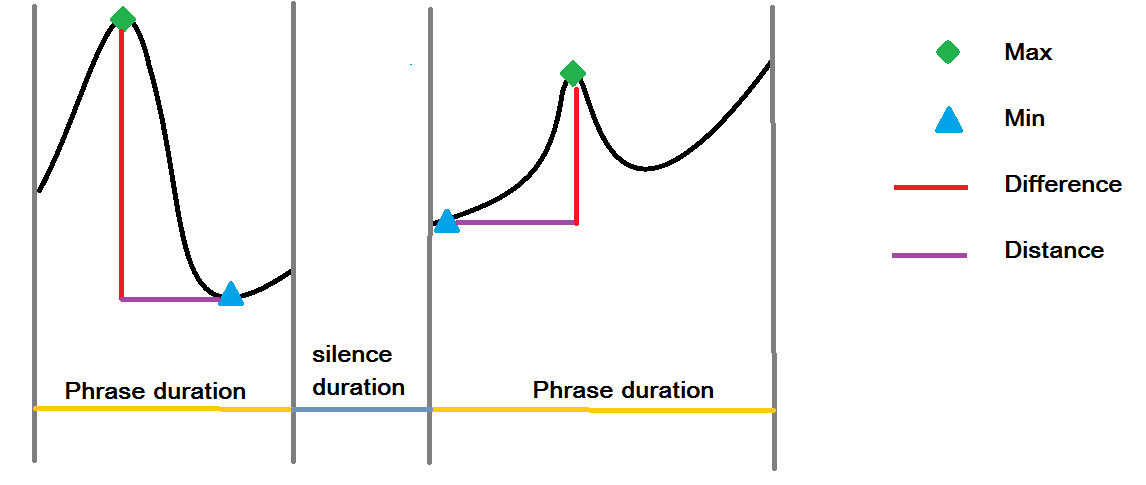
\includegraphics[scale=0.5]{images/dds.png}
	\caption{DDS}
	\label{fig:dds}
\end{figure}
Phrase duration and silence duration are calculating by phrase pointers. Also, center of gravity of spectrogram for all speech provides PRAAT library. So for each record is extracted features represented in the Table 2.
\subsection{Features from training data set}
For further building a classifier is necessary to identify relations between these features and emotions. It requires a training set with split emotional speech records. 

But before, should be selected emotions for recognition. A recognizable set of emotion is important for the system's accuracy. In this work will be used four emotions: \emph{anger, happiness, sadness and neutral}. Because these emotions are basic and they are more clearly expressed in human speech.

There are many databases of emotional speech. And they differ in:
\begin{itemize}
	\item number of emotions
	\item number of actors (speakers)
	\item nature of emotion (artificially played or really expressed emotions)
	\item number of various texts
\end{itemize}
"EmoDB"\cite{emodb} - german database of emotions will be used. It consists of emotional records spoken by 10 different actors. They express 7 emotions (anger, boredom, disgust, fear, happiness, sadness, neutral), but we will use only four emotions which we selected above. Each actor expresses an emotion with a several texts. For our goals this database contains 107 speech records. For each speech we calculated features, and for selected emotions was taken medians for each feature. So results of extracted features from training data set are represented in the Table 3.
\begin{table}[h]
	\centering
		\begin{tabular}{l|l|l|l|l|}
			\hline
				Feature/Emotion& anger&	happy	&sadness	&neutral\\ \hline
PitchDff&	137,08	& 211,55	&67,32	&64,63\\ \hline 
PitchDis&	-6	&-10,125&	-19,33&	-8\\ \hline
IntDif&	22,22&	22,92&	19,63&	18,76\\ \hline
IntDis	&6,44	&-5,83&	-7,41&	-3,2\\ \hline
F1Dif&	239,44&	228,16&	210,52&	193,49\\ \hline
F1Dis&	-1,71	&-5,87&	-9&	-1,66\\ \hline
F2dif	&349,82&	318,56&	340,58&	299,02\\ \hline
F2Dis&	-1,42&	-3,15&	-2,32	&0,66\\ \hline
F3Dif&	355,51&	359,38&	449,35&	425,46\\ \hline
F3Dis&	-0,4	&-2,28&	-0,33&	2,6\\ \hline
PitchRange&	465,16&	406,37&	150,065&	457,2\\ \hline
IntRange&	31,36&	28,95&	28,865&	27,61\\ \hline
PitchVariance&	7253,96&	10823,92&	1737,46&	6720,77\\ \hline
IntVariance	&46,19&	41,20&	35,10	&36,24\\ \hline
PhraseDuration&	28,9&	38,16&	39,58	&24,66\\ \hline
SilenceDuration	&5,2	&4,45	&5,375&	5,4\\ \hline
Centroid&	580,3	&519,54&	359,08&	350,02\\ \hline
 \hline
		\end{tabular}
	\caption{Extracted features from training data set. Dif-Difference, Dis-Distance, Int-Intensity}
	\label{tab:ExtractedFeaturesFromTrainingDataSet}
\end{table}

\subsection{Classification}
So we have got some feature values for each emotion, and is needed to build classifier using them. Each feature has 4 values which mapped with emotions. Therefore each emotion can be characterized by set of approximate values of features. For example, PitchDiff has values: 	137,08;  211,55; 67,32; 64,63; 

Problem here is how to identify that some value is closer to one of the feature value. It is impossible to set strict confines of feature
values for each emotion. In addition, some feature values are very similar and it's difficult divide them to four classes. But often among these 4 values exist two high and two low values. It caused by fact that some emotion very similar with some features, but they have some distinct features.
For example: angry-happy, sadness-neutral. It can be seen on the Table 3, most of the features of angry and happiness are similar, but there are some features which distinct for them. For example, phrase duration is lower for anger.

That is why was decided to use fuzzy sets for classifying each feature to two classes: \emph{high} and \emph{low} triangle membership function.  Because classification to 2 classes will be more precise. And fuzzy sets allow to set intersection between them.
\begin{figure}[t]
	\centering
		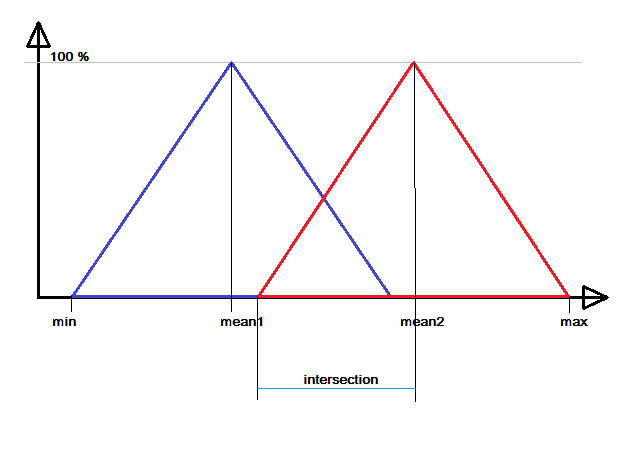
\includegraphics[scale=0.7]{images/fuzzy-sets.png}
	\caption{Fuzzy sets}
	\label{fig:fuzzy-sets}
\end{figure}

\subsubsection{Fuzzy sets construction}
So we have to construct two fuzzy sets from 4 feature values. In addition, for each feature is necessary determine $min$ and $max$ values. Each set represented as a triangle. At the top of the triangle membership probability is equal to 100\%. 

Algorithm is as follows:

\begin{enumerate}
	\item Sort values of feature
	\item $mean1=$ average value of two first values, $mean2=$ average value of two last values
	\item $intersection=$ 20\% of maximum element (first element)
	\item first set is= $\{ (min,0) , (mean1, 100) , (mean2-intersection, 0) \}$, second set is= $\{ (mean1+intersection, 0), (mean2, 100) , (max, 0) \}$
\end{enumerate}

Example with centroid values $\{580,3;519,54;359,08;350,02\}$\\
\[ sorting    \{580.3;519.54;359.08;350.02\} \]\\
\[ mean1=\frac{580.3+519.54}{2} \]
\[ mean2=\frac{359.08+350.02}{2}\]
\[intersection=\frac{580.3*20}{100}\]

Now is necessary define $min$ and $max$ values of this feature. Centroid is the center of mass for spectrum. Spectrum is representation of signal in frequency domain. And because fundamental frequency of human voice approximately  located between 30 and 1000 Hz. $min$ values for centroid is 30 and $max$ is 1000.

All features related with frequency range have such min and max values:
\begin{itemize}
	\item PitchDiff
	\item F1Dif, F2Dif, F3Dif
	\item PitchRange
	\item Centroid
\end{itemize}
For other features $min$ and $max$ values was set on the basis of the spread of the values.

Eventually, we have got 5 values for two fuzzy sets construction. For each feature we can define two characterizing functions: $IsLow$ and $IsHigh$, which will return probability. And based on this model from training data set each emotion can be described as in the Table 4. So, accuracy of classification depends on properly selected fuzzy sets boundaries.


\begin{table}[h]
	\centering
		\begin{tabular}{l|l|l|l|l|}
			\hline
				Feature/Emotion& anger&	happy	&sadness	&neutral\\ \hline
PitchDff&	High	&High	&Low	&Low\\ \hline 
PitchDis&	High	&Low&	Low&	High\\ \hline
IntDif&	High&	High&	Low&	Low\\ \hline
IntDis	&High	&Low&	Low&	High\\ \hline
F1Dif&	High&	High&	Low&	Low\\ \hline
F1Dis&	High	&Low&	Low&	High\\ \hline
F2dif	&High&	Low&	High&	Low\\ \hline
F2Dis&	High&	Low&	Low	&High\\ \hline
F3Dif&	Low&	Low&	High&	High\\ \hline
F3Dis&	Low	&Low&	High&	High\\ \hline
PitchRange&	High&	High&Low&	Low\\ \hline
IntRange&	High&	High&	Low&	Low\\ \hline
PitchVariance&	High&	High&Low&	Low\\ \hline
IntVariance	&High&	High&	Low	&Low\\ \hline
PhraseDuration&	Low&	High&	High	&Low\\ \hline
SilenceDuration	&Low	&Low	&High&	High\\ \hline
Centroid&	High	&High&	Low&	Low\\ \hline
 \hline
		\end{tabular}
	\caption{}
	\label{tab:}
\end{table}

And the emotion probability computing will look like:\\ $anger=PitchDif.IsHigh() + PitchDis.IsLow() + IntDif.IsHigh() + ...$

So this classifier is obtained similar to Binary decision tree but with fuzzy logic. Both have simple implementation, fast classification, fast learning, make changes after learning is possible.
\subsection{System as whole}

\begin{figure}[h]
	\centering
		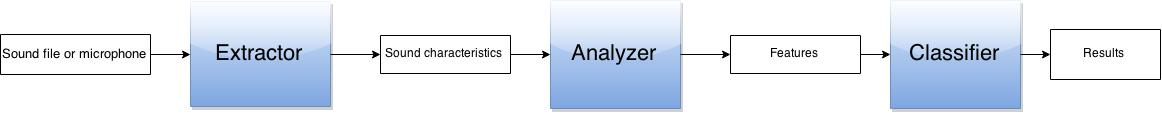
\includegraphics[scale=0.3]{images/components.png}
	\caption{System as a whole}
	\label{fig:system}
\end{figure}

System's work as whole shown in the Figure 7. Extractor receives sound from file or microphone and extracts sound characteristics using PRAAT. Then Analyzer computes features for sound characteristics for further classification. Classifier using fuzzy sets computes probability for each emotion.

\section{Testing}
Before considering the results of our implementation, is necessary to note some points about on what depends accuracy. As mentioned above, accuracy of the system depends on used features and classifier. But also it depends on training data set and data set used to test. Because there is real ambiguity between expressed emotions. Also, EmoDB contains only artificially expressing emotions. So, some actors can express emotions ambiguously. More dependent on talk context and on person specific manner of speaking. It can be proved by results of human performance in emotion recognition (Figure 8) from \cite{frankthomas} paper.
\begin{figure}[h]
	\centering
	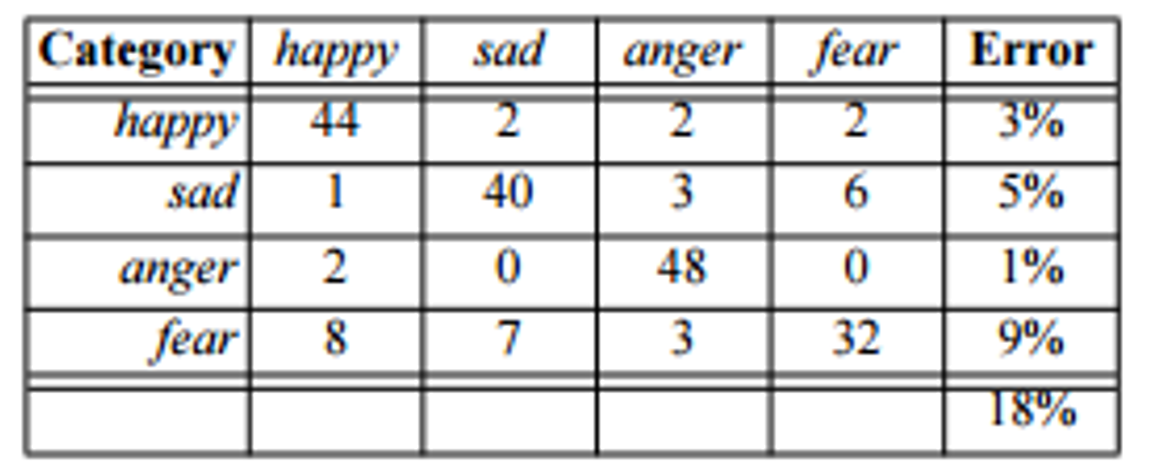
\includegraphics[scale=0.3]{images/h_performance.png}
	\caption{}
	\label{fig:human-perforance}
\end{figure}

\subsection{Test results with training data set}

\begin{table}
	\centering
	\begin{tabular}{|l|l|l|l|l|}
		\hline
		&anger&happy&sadness&neutral\\ \hline
		anger&\textbf{55}&16&9&18\\\hline
		happy & 17 & \textbf{47} & 11 & 23 \\\hline
		sadness & 3 & 11 & \textbf{62} & 22\\\hline
		neutral & 20 & 15 & 15 & \textbf{51}\\\hline
		
	\end{tabular}
	\caption{Restults for training data set}
\end{table}
\begin{table}[h]
	\centering
	\begin{tabular}{|l|l|l|l|}
		\hline
		&anger&happy&sadness\\ \hline
		anger&\textbf{60}&34&4\\\hline
		happy & 35 & \textbf{64} & 0\\\hline
		sadness & 7 & 33& \textbf{59}\\\hline
		
	\end{tabular}
	\caption{Restults for training data set without neutral emotion}
\end{table}
As we can see in the Table 5, the most precisely recognized sadness and anger, i.e. passive and active emotions. Table 6 where represented results without neutral emotions, shows that accuracy can be better. And neutral emotion can be deduced from analyzing other emotions values. For example, if values of anger, happiness and sadness are very close, it means that speech is neutral.

\subsection{Testing with test (other) data set}
Draw conclusions on the basis of testing results on trainning set is not entirely correct. That is why for testing was recorded other emotional speech files. Note that training set consist of records of german speech. This set contains english and russian languages. 
\section{Conclusions and further work}
According to the results of testing we can see: influence to accuracy have not only used features and classification methods, but also selected emotions for recognition. It confirms that recognizable emotions should be chosen specially for application domain of the system. For example, in some cases is needed only active-passive or positive-negative emotions recognition, and it can be more precise, as shown in testing results.

Of course, in our simple implementation wasn't used MFCC or other characteristic which can be useful. In addition, classification technique (some mix of Fuzzy sets and Binary decision tree) is not ideal, and for better results can be used another classificator.

But the main goal of this work in considering of studies and implementation solution. Our simple solution has some advantages and disadvantages:\\\\
\textit{Advantages:}
\begin{itemize}
	\item noise removing
	\item dividing speech to phrases
	\item fast learning (the main part of time spent for sound characteristics extraction, classifier learning is done very fast)
\end{itemize}
\textit{Disadvantages:}
\begin{itemize}
	\item accuracy is very strongly associated with training set. 
	\item dividing speech to phrases would be wrong with unfiltered noises
	\item fuzzy sets have $min$ and $max$ confines
\end{itemize}

\subsection{Further work}
So, for further work is necessary to consider these aspects: sound characteristics, features, classification and testing.

\subsubsection{Sound characteristics}
Besides pitch, loudness, formant can be used MFCC, or spectral characteristics. But is necessary to  make sure of need spectral characteristics, because it requires more time for calculating. That is why for speech recognition often used MFCC.

\subsubsection{Features}
Among of all features is necessary select ones which have less dependence with person specifics, recording context. For universal using of the system they should describe speech signal dynamics. In addition is necessary to find out weight of each feature, in other words it's contribution to classification result.

\subsubsection{Classification and testing}
Further can be done:
\begin{itemize}
	\item classifier training with other training set and comparing results. There are many databases of emotional speech.
	\item use other classifier(k-NN, SVM, ANN) and compare accuracy
	\item classification to classes: postive-nagative, passive-active. Because it may be more precise
	\item try various combinations of classifier and set of emotions
\end{itemize}
\begin{thebibliography}{9}

\bibitem{affective}
"Affective computing",
http://en.wikipedia.org/wiki/Affective\_computing

\bibitem{pepper}
"Pepper",
https://www.aldebaran.com/en/a-robots/who-is-pepper

\bibitem{wiki1}
Fundamental frequency,
http://en.wikipedia.org/wiki/Fundamental\_frequency

\bibitem{wiki2}
Formant,
http://en.wikipedia.org/wiki/Formant

\bibitem{wiki3}
Mel-frequenc cepstrum
http://en.wikipedia.org/wiki/Mel-frequency\_cepstrum

\bibitem{wiki_loudness}
Sound loudness,
http://en.wikipedia.org/wiki/Loudness


\bibitem{SirishaSirvinasSiva}
"Speaker Emotion Recognition Based on Speech Features and Classification Techniques",
J. Sirisha Devi, Dr. Srinivas Yarramalle, Siva Prasad Nandyala\\
I.J. Computer Network and Information Security, 2014, 7, 61-77

\bibitem{brittaelizabet} "Real-time automatic emotion recognition
from speech",
 Dr. Britta Wrede, Prof. Dr. Elisabeth André, 2010

\bibitem{emodb}"EmoDB" Felix Burkhardt, Astrid Paeschke, Miriam Rolfes, Walter Sendlmeier und Benjamin Weiss
A Database of German Emotional Speech
Proceedings Interspeech 2005, Lissabon, Portugal\\
http://www.emodb.bilderbar.info/.

\bibitem{pierre}"The production and recognition of emotions in
speech: features and algorithms",
 Pierre-Yves Oudeyer,Int. J. Human-Computer Studies 59 (2003) 157–183

\bibitem{praat} "PRAAT",
 Paul Boersma and David Weenink   
Phonetic Sciences, University of Amsterdam//
http://www.fon.hum.uva.nl/praat/

\bibitem{frankthomas}"Recognizing emotion in speech",
Frank Dellaert, Thomas Polzin and Alex Waibel. Carnegie Mellon University. 


\end{thebibliography}
\end{document}
